\chapter{Návrh systému a Implementácia}
V tejto kapitole sa venujeme stručnému opisu návrhu systému a jeho jednotlivých častí a taktiež opisujeme kľúčové prvky implementácie.

Pri návrhu a implementácii našej aplikácie sme brali do úvahy výhody a obmedzenia systému \textit{IMS4} (\textit{Integrated Monitoring System}), ktorý je vyvíjaný spoločnosťou \textit{MicroStep-MIS s.r.o.}. Dôvodom je, že náš verifikačný systém bol navrhovaný ako prídavný modul pre spomenutý systém IMS4.

\section{Návrh systému}
\label{sec:sysdesign}
Našu aplikáciu sme sa snažili navrhnúť ako samostatný produkt schopný extrakcie a spracovania meteorologických dát a výpočtu verifikačných štatistík, ale taktiež aj ako súčasť systému IMS4. Toto sme dosiahli tak, že sme rozdelili systém na 2 balíky: \textit{verifikačný} a \textit{vizualizačný}. Na obrázku \ref{fig:system} môžeme vidieť schematický návrh systému.

\textit{Verifikačný balík} tvorí jadro celého systému a zohráva viacero úloh. V prvom rade je jeho úlohou extrakcia dát z rôznych dátových zdrojov do tabuliek predpovedí a pozorovaní. Tieto tabuľky sa následne predspracúvajú (párovanie, konverzia fyzikálnych jednotiek, filtrovanie, identifikácia chýbajúcich dát...) a posúvajú sa do časti na výpočet štatistík. Na základe konfigurácie sa spočítajú rôzne štatistiky, ktorých výsledok je výstupom z tohoto balíka.

\pagebreak

\textit{Vizualizačný balík} chápeme ako vymeniteľnú časť systému. Vďaka tomuto môže byť vizualizácia v podobe interaktívnej obrazovky, ktorá je súčasťou systému IMS4, ale taktiež generovaná automaticky do statických obrázkov na disku.

\begin{figure}
	\centering
	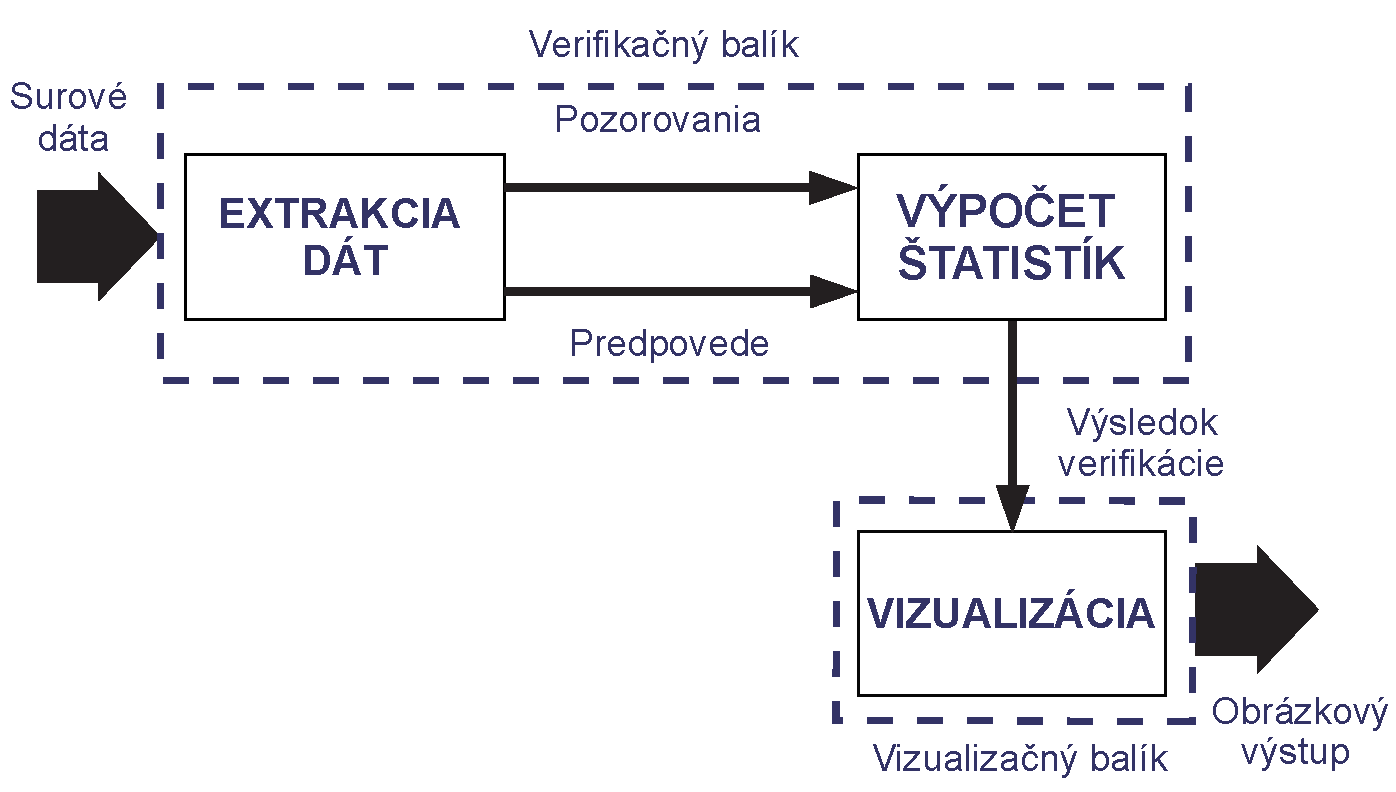
\includegraphics[width = 5in]{system}
	\caption{Schematický popis systému.}
	\label{fig:system} 
\end{figure}

Ak by sme mali systém opísať v pojmoch vizualizácie informácií, tak tieto dva balíky rozdeľujú vizualizačnú \textit{pipeline} na dve časti (Pozri obrázok \ref{fig:pipeline}). Verifikačný balík sa stará o analýzu dát pomocou predspracovania a matematického modelu verifikačných štatistík a taktiež sa stará o filtrovanie dát. Zvyčajne filtrovanie prebieha na základe interakcie užívateľa. V našom prípade sme však uvažovali aj o možnosti, že vizualizácia nebude interaktívna, preto sme filtrovanie umiestnili do verifikačného balíka a vykonáva sa na základe konfigurácie systému. 

Filtrované dáta putujú do vizualizačného balíka. V ňom sa vykonáva zobrazenie hodnôt na vizuálne parametre jednotlivých prvkov vizualizácie, tak ako sme to opísali v kapitole \ref{chap:design} \textit{Návrh vizualizácie}. Takéto dáta sa následne vykreslia do obrázka alebo na obrazovku, čím sa ukončí vizualizačná pipeline.

\begin{figure}
	\centering
	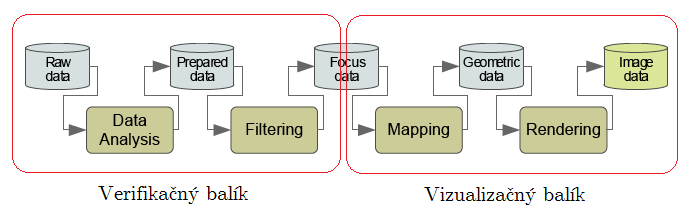
\includegraphics[width = 6in]{pipeline}
	\caption{Rozdelenie prvkov vizualizačnej pipeline do verifikačného a vizualizačného balíka. Obrázok pipeline pochádza zo stránky \protect\url{http://www.infovis-wiki.net}.}
	\label{fig:pipeline} 
\end{figure}


\section{Použité technológie}
Výber implementačných nástrojov bol podmienený obmedzeniami systému IMS4. Z tohto dôvodu sa návrh jednotlivých častí odvíja čiastočne aj od použitej technológie a aj preto uvádzame v našej práci sekciu \textit{Použité technológie} skôr, ako samotný návrh jednotlivých balíkov.

\subsection{Java}
Primárnu časť systému - \textit{verifikačný balík} sme implementovali v jazyku \textit{Java}, konkrétne vo verzii 1.5. Toto je prvé obmedzenie, ktoré na nás kladie systém IMS4, keďže použitie vyššej verzie (momentálne je dostupná už verzia 1.8) by spôsoboval problém s kompatibilitou.

Java ako programovací jazyk je veľmi rozšírený a obľúbený, vďaka čomu je dostupné pomerne veľké množstvo knižníc, nevynímajúc originálne knižnice zahrnuté v systéme IMS4. Tieto knižnice sme využili pri implementácii aj my. Môžeme spomenúť 3 knižnice, z ktorých sú dve interné a jedna pôvodne externá s pridanou funkcionalitou. Prvé dve spomenuté sú \textit{Log} - používaná na logovanie a \textit{X2O}, ktorá sa používa na mapovanie javovských objektov na XML štruktúru a späť pomocou \textit{Java Reflection API}. My sme X2O použili pri ukladaní a načítavaní konfiguračných súborov. Posledná knižnica je \mbox{NetCDF-grib} \cite{Unidata} a pochádza od americkej organizácie \textit{Unidata}, ktorú zastrešuje \textit{UCAR}. Jedná sa o opensource produkt na čítanie dát zo súborov vo formáte GRIB. My využívame upravenú verziu NetCDF-grib-6.0 obzvlášť kvôli Jave 1.5, aj keď sú dostupné novšie verzie\footnote{Najnovšia je NetCDF-Java-4.5, ktorá zoskupuje všetky ďalšie podobné produkty od Unidata.}.

\subsection{JavaScript}
Systém IMS4 využíva webové stránky na vytváranie GUI. Z tohto dôvodu sme sa rozhodli, že vizualizáciu budeme produkovať priamo v prehliadači pomocou \textit{JavaScriptu}. Podobne ako Java, aj JavaScript je veľmi populárny a preto vzniklo veľké množstvo rôznych knižníc, medzi ktorými sú aj mnohé určené na vizualizáciu. K najznámejším z nich patria napríklad: \textit{JavaScript InfoVis Toolkit}, \textit{Highcharts}, \textit{jQuery Visualize}, \textit{JS Charts}, \textit{jqPlot}, \textit{jpGraph}, \textit{Raphaël}, \textit{Dygraphs},\textit{ Processing.js}, \textit{Axiis}, \textit{D3} a mnohé ďalšie. Pre naše účely sme z veľkého množstva knižníc vybrali práve D3, ako pre nás najvhodnejší nástroj.

\subsubsection{D3}
D3 (\textit{Data-Driven Documents}) \cite{D3} je opensource knižnica napísaná v JavaScripte. Na vizualizáciu využíva HTML a SVG elementy a ich vizuálne vlastnosti, ktoré mení pomocou ich atribútov a CSS štýlov. 

Dôvodom, prečo sme si vybrali práve D3 z veľkého množstva vizualizačných knižníc je, že väčšina z nich bola zameraná na konkrétny druh vizualizácie (napr. \textit{force-directed layout}) alebo na niekoľko najpoužívanejších druhov diagramov (bodový, stĺpcový, čiarový, histogram,...). D3 sa však nezameriava na konkrétny druh vizualizácie, ale ponúka spôsob, ako zobrazovať hodnoty na vizuálne parametre elementov, čím umožňuje ohromnú variabilitu a je vhodná na vytváranie nových alebo menej používaných typov vizualizácií. Väčšina vizualizácií, ktoré sme v našej práci navrhli, nie sú podporované vyššie spomenutými knižnicami a preto sme potrebovali nástroj umožňujúci dobre parametrizovateľnú vizualizáciu.

Toto je taktiež dôvod, prečo vzniklo veľké množstvo knižníc, ukážkových príkladov a návodov ktoré využívajú práve knižnicu D3. Aby sme spomenuli aspoň niektoré z knižníc používajúcich D3, tak sú to napríklad \textit{Raw}, \textit{Cubism}, \textit{Ember Charts}, \textit{NVD3}, \textit{C3}, \textit{MetricsGraphics}, \textit{Graffeine}, \textit{Mermaid}, \textit{Epoch}, \textit{Insights}, \textit{Dashku}, \textit{RickShaw} a mnohé ďalšie. 

\section{Verifikačný balík}
Ako sme už spomenuli v sekcii \ref{sec:sysdesign} , tento balík sa skladá z dvoch logických častí: \textit{Spracovanie dát} a \textit{Výpočet štatistík}. V tejto sekcii sa pokúsime zhrnúť kľúčové prvky návrhu a implementácie týchto dvoch častí.
\subsection{Spracovanie dát}
Úlohou tejto časti je získanie potrebných dát z určených dátových zdrojov a ich predspracovanie tak, aby mohli vstúpiť do ďalšej časti - \textit{Výpočet štatistík}.

Pri návrhu tried na získavanie predpovedí a pozorovaní sme sa snažili, aby bolo užívateľovi umožnené získavať dáta z viacerých typov zdrojov: Gribovské súbory, CSV súbory, webové zdroje, databáza a podobne. Aby sme pre každý typ zdroju nevytvárali samostatnú vetvu udalostí, navrhli sme abstraktnú triedu \textit{DataExtractor}, ktorá obsahuje abstraktné metódy \texttt{extract()} a \texttt{addSoruces()} a taktiež slúži na inštancovanie všetkých jej potomkov (pozri UML diagram na obrázku \ref{fig:dataextractor}). Jednotlivý potomkovia následne musia implementovať vyššie spomenuté metódy, ktoré sú špecifické pre každý typ zdroju. Napríklad pre webové zdroje metóda \texttt{addSoruces()} očakáva url adresu, zatiaľ čo pre dátové súbory očakáva cestu.

Z extrakcie dát získame tabuľky hodnôt s pozorovaniami a predpoveďami pre konkrétne časy. Tieto dáta sa následné predspracúvajú v štyroch krokoch:

\begin{enumerate}
	\item \textit{Párovanie} : Prebieha tak ako je opísané v podsekcii \ref{subsec:pairing}.
	\item \textit{Filtrovanie} : Na základe konfigurácie získavame iba dátumy zvolené užívateľom.	\item \textit{Konverzia jednotiek} : Fyzikálne jednotky z predpovedí a pozorovaní konvertujeme do rovnakej jednotky podľa konfigurácie, aby bol výpočet chýb korektný.
	\item \textit{Výpočet chýb} : Prebieha tak ako je opísané v sekcii \ref{sec:errormeasurement}.
\end{enumerate}

\noindent Tak ako je naznačené na obrázku \ref{fig:system},  takto spracované dáta putujú do časti výpočet štatistík.

\begin{figure}
	\centering
	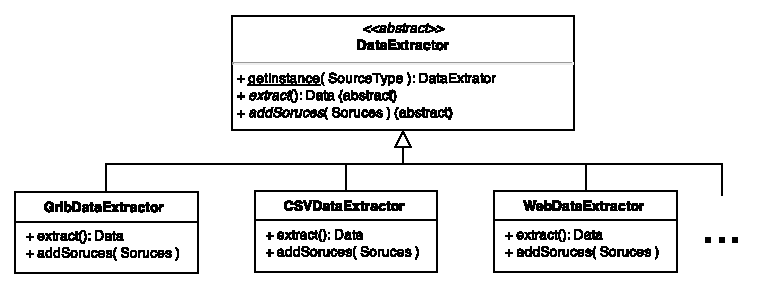
\includegraphics[width = 6in]{dataextractor}
	\caption{Triedny UML diagram pre triedy typu DataExtractor.}
	\label{fig:dataextractor} 
\end{figure}

\subsection{Výpočet štatistík}
V tejto časti verifikačného balíka sa vykonáva výpočet štatistík, ktoré sme opísali v sekcii \ref{sec:errormeasurement}. V nej sme taktiež navrhli vzorec, ktorý opisuje výpočet kumulovanej chyby vo všeobecnosti pomocou dvoch funkcií $ \varepsilon $ a $ \Phi $ (pozri podsekciu \ref{subsec:cumulativeerror}).


Pre pripomenutie, funkcie $ \varepsilon $ a $ \Phi $ sú ľubovoľnými funkciami z $\mathbb{R}$ do $\mathbb{R}$ a všeobecný vzorec pre kumulované skóre je nasledovný: $ \Phi(\sum\limits_{i=0}^{n} \varepsilon(e_i)) $. Ako vidíme $ \varepsilon $ slúži na spracovávanie chyby a $ \Phi $ na spracovávanie sumy. Toto riešenie sme použili aj pri návrhu a implementácii programových tried na výpočet štatistík. Na obrázku \ref{fig:stats} môžme v triednom diagrame vidieť, že hlavným telom celého návrhu je abstraktná trieda \textit{ContinuousStatistics} obsahujúca dve abstraktné metódy \texttt{processError()} a \texttt{processSum()}. Práve tieto dve metódy predstavujú funkcie $ \varepsilon $ a $ \Phi $. Trieda \textit{ContinuousStatistics} obsahuje taktiež tretiu - \textit{nie abstraktnú} - metódu \texttt{calculateStatistics()}, v ktorej tele sa vykonáva suma všetkých chýb s použitím týchto dvoch metód. Na obrázku \ref{fig:stats} môžme taktiež vidieť, že všetky štatistiky sú implementované ako potomkovia triedy \textit{ContinuousStatistics} a teda musia implementovať vyššie spomenuté abstraktné metódy. To ako vyzerajú tieto metódy pre jednotlivé štatistiky sme taktiež ukázali v spomínanej podsekcii \ref{subsec:cumulativeerror}.

 \pagebreak 
             
\begin{figure}
	\centering
	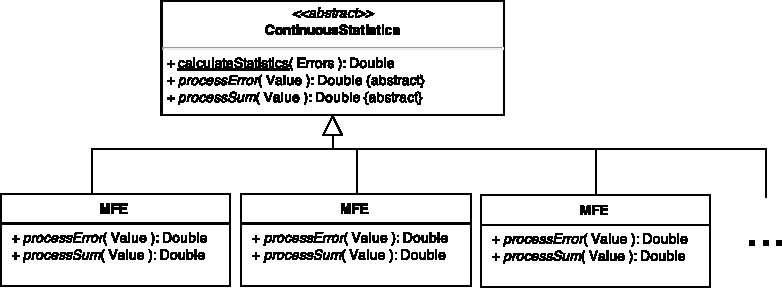
\includegraphics[width = 5in]{stats}
	\caption{Triedny UML diagram pre triedy typu ContinuousStatistics.}
	\label{fig:stats} 
\end{figure}

\section{Vizualizačný balík}
Úlohou vizualizačného balíka je spracovávanie výsledkov verifikácie a vygenerovanie z týchto dát obrazovku vizualizácie navrhnutú v predošlej kapitole. 

Pri návrhu a implementácii tohto balíka sme sa snažili využiť niektoré vlastnosti, ktoré nám ponúkajú použité technológie. Veľkú časť tohto balíka sme navrhli ako súčasť knižnice D3 s vyžitím návrhových vzorov charakteristických pre túto knižnicu. Jednak išlo o takzvaný \textit{chaining pattern}, ktorý slúži pri vytváraní objektu. Tento pattern dovoľuje volanie metód objektu, ktorými sa nastavujú jeho vlastnosti, zreťazených za sebou. Príklad pre lepšie pochopenie je ukázaný na výpise \ref{list:chaining}.
Ďalším vzorom je \textit{callback pattern}, kedy sa používa funkcia ako parameter. 


\begin{lstlisting}[frame=solid, backgroundcolor=\color{bg}, basicstyle=\footnotesize\ttfamily, language=JavaScript, numbers=left, numberstyle=\tiny\color{black}, caption=Ukážka aplikácie návrhového vzoru \textit{chainning}., captionpos=b, label=list:chaining]
var groups = group.selectAll(".group")
		    .data(data)
		    .enter()
		    .append("svg:g")
		    .classed("group", true);	
\end{lstlisting}

Jednotlivé prvky vizualizácie sme navrhli ako takzvané \textit{moduly}, ktoré obsahujú v sebe dáta, nastavenia zobrazenia a ďalšie vnorené moduly, ako svojich potomkov. Každý modul je funkcia, ktorá ma na vstupe \textit{selection}, teda DOM element vybraný pomocou knižnice D3. Tento typ funkcie je \textit{callback} funkcia, ktorú jednotlivé vybrané elementy knižnice D3 volajú pomocou metódy \texttt{call()}. 

Tento návrh nám vytvára akúsi stromovú štruktúru modulov (pozri obrázok \ref{fig:tree}), ktorá umožňuje jednoduché vystavovanie celého rozloženia prvkov, kombinovanie jednotlivých častí vizualizácie a znovupoužitie niektorých častí vizualizácie. 

Príkladom znovupoužitia môže byť graf pre distribúciu chýb, ktorý sa skladá z horizontálnej a vertikálnej osi a samotnej vizualizácie, ktorá môže byť rôzna (pozri sekciu \ref{sec:distribdesign}). Pre rôzne typy vizualizácií teda nemusíme kopírovať rovnaký kus kódu na generovanie osí viackrát, ale iba recyklujeme opakujúcu sa časť grafu.   

Každý typ grafu sme taktiež rozobrali na základné časti, z ktorých sa skladá. Napríklad mnoho-čiarový diagram sa skladá z osí, horizontálnej a vertikálnej mriežky a mnohých čiar. Vďaka tomuto jednak môžme jednoducho riadiť počet čiar alebo mriežok, ale taktiež môžme čiarový diagram kombinovať so stĺpcovým, s bodovým alebo ľubovoľným iným diagramom. Zjednodušene povedané, tým, že každý element chápeme ako samostatný modul, získavame dobrú variabilitu vizualizácie.

\begin{figure}
	\centering
	\hspace*{-0.2in}
	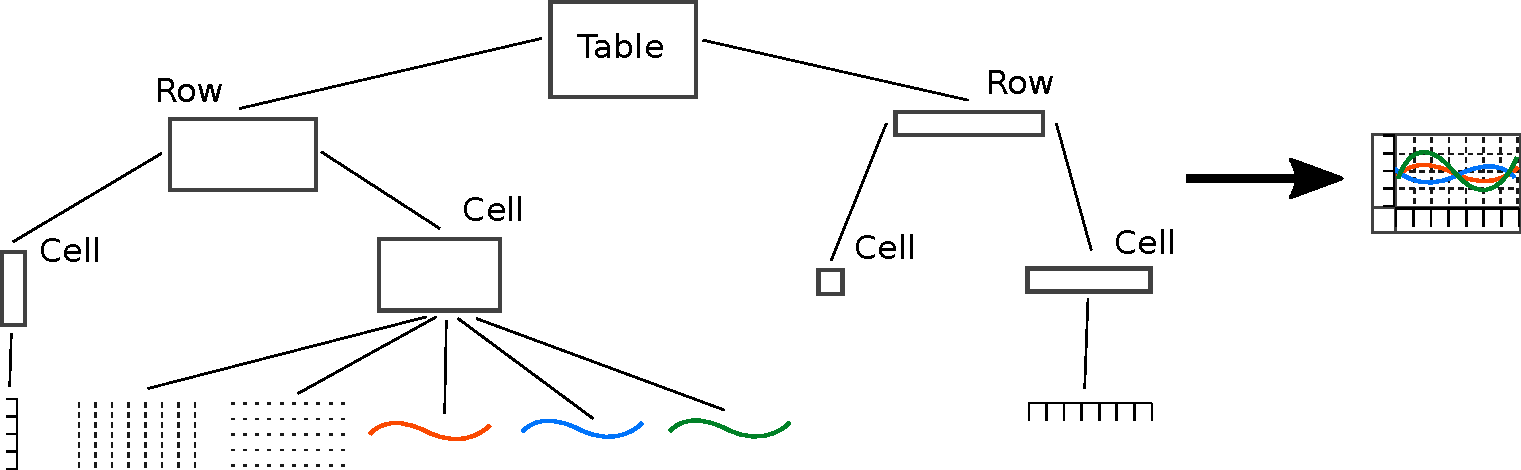
\includegraphics[width = 6in]{tree}
	\caption{Príklad štruktúry modulov pre vytvorenie mnoho-čiarového diagramu.}
	\label{fig:tree} 
\end{figure}